\documentclass[a4paper,12pt]{ctexart}
\usepackage{amsmath}
\usepackage{amssymb}
\usepackage{fontspec}
\usepackage{xeCJK}
\usepackage{graphicx}
\usepackage{listings}
\usepackage{xcolor} 
\usepackage{graphicx}
\usepackage{booktabs} %绘制表格
\usepackage{geometry}
\usepackage{array}
\usepackage{longtable}
\usepackage{abstract}
\usepackage{caption}
\usepackage{subcaption}
\usepackage{abstract}
\usepackage{makecell}
\usepackage{float}
%防止表格乱跑:[H]
\usepackage{listings}
%添加代码块
\usepackage{fancyhdr} 
%导入fancyhdr包
\usepackage{threeparttable}
%给代码添加注释

\lstset{
 numbers=left, %设置行号位置
 numberstyle=\tiny, %设置行号大小
 keywordstyle=\color{blue}, %设置关键字颜色
 commentstyle=\color[cmyk]{1,0,1,0}, %设置注释颜色
 escapeinside=``, %逃逸字符(1左面的键),用于显示中文
 breaklines, %自动折行
 extendedchars=false, %解决代码跨页时,章节标题,页眉等汉字不显示的问题
 xleftmargin=1em,xrightmargin=1em, aboveskip=1em, %设置边距
 tabsize=4, %设置tab空格数
 showspaces=false %不显示空格
}

\lstset{
 columns=fixed,       
 numbers=left,                            % 在左侧显示行号
 numberstyle=\tiny\color{gray},           % 设定行号格式
 frame=none,                              % 不显示背景边框
 backgroundcolor=\color[RGB]{245,245,244},% 设定背景颜色
 keywordstyle=\color[RGB]{40,40,255},     % 设定关键字颜色
 numberstyle=\footnotesize\color{darkgray},           
 commentstyle=\it\color[RGB]{0,96,96},    % 设置代码注释的格式
 stringstyle=\rmfamily\slshape\color[RGB]{128,0,0},   
            % 设置字符串格式
 showstringspaces=false,                  % 不显示字符串中的空格
 language=matlab,                         % 设置语言
}

\setlength{\parindent}{2em} %2em代表首行缩进两个字符
\pagestyle{headings}
\pagestyle{fancy}
% 页眉设置
\fancyhead{} % 初始化页眉
\fancyhead[L]{Matlab仿真实验1}
\fancyhead[R]{3200104845}
\fancyhead[C]{朱少廷}
\fancyfoot{} % 初始化页脚
\fancyfoot[L]{}
\pagenumbering{Alph}%设置页码格式
\renewcommand{\headrulewidth}{1.5pt}%分隔线宽度4磅

\setlength{\absleftindent}{0pt}
\setlength{\absrightindent}{0pt}


\graphicspath{{pictures/}}

% Set page size and margins
\geometry{a4paper,top=3cm,bottom=2cm,left=3cm,right=3cm,marginparwidth=1.75cm}

\begin{document}
\centerline{\Large{\textbf{Matlab仿真实验1}}}
\leftline{\textbf{实验目的:}}

\begin{itemize}
    \item 了解连续时间信号的基本概念及其运算实现。
    \item 熟悉 Matlab 编程特点,建立对连续时间信号及其频谱的直观认识。
\end{itemize}

\leftline{\textbf{实验内容:}}
\leftline{1.产生并画出以下信号}
(1)单位冲激函数
\begin{equation}
    \delta (t)=\lim_{\tau \rightarrow 0}\frac{1}{\tau }(u(t+\frac{\tau }{2})-u(t-\frac{\tau }{2}))
\end{equation}

\begin{lstlisting}
%% Unit impulse signal
t=-5:0.01:5;
k=1e-10;
y=1/k.*(heaviside(t+k/2)-heaviside(t-k/2));
plot(t,y);
ylim([-2 2]);
\end{lstlisting}
\begin{figure}[H]
    \centering
    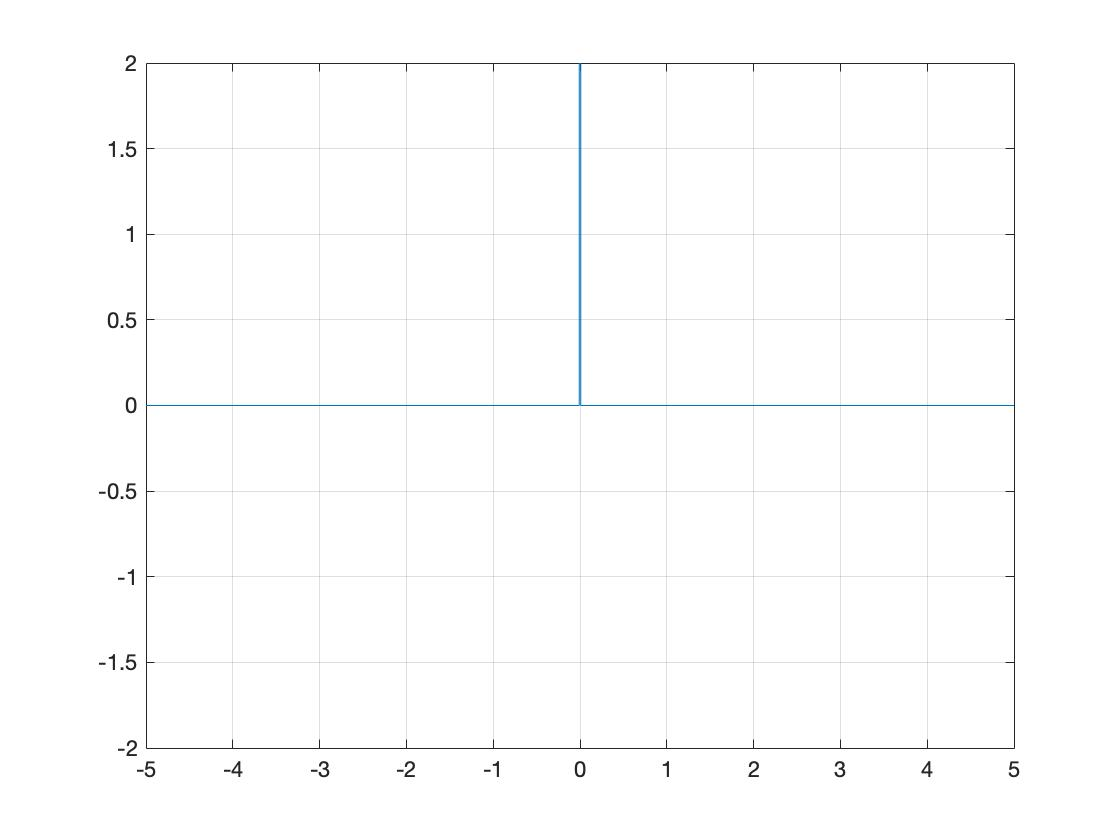
\includegraphics[width=14cm]{1.jpg}
    \caption{单位冲激函数}
\end{figure}

(2)单位阶跃函数
\begin{equation}
    u(t)=\left\{\begin{matrix}
        1 & t>0 \\
        0 & t<0
    \end{matrix}\right.
\end{equation}

\begin{lstlisting}
%% Unit step function
t=-5:0.01:5;
y=stepfun(t,0);
plot(t,y);
ylim([-2 2]);
\end{lstlisting}
\begin{figure}[H]
    \centering
    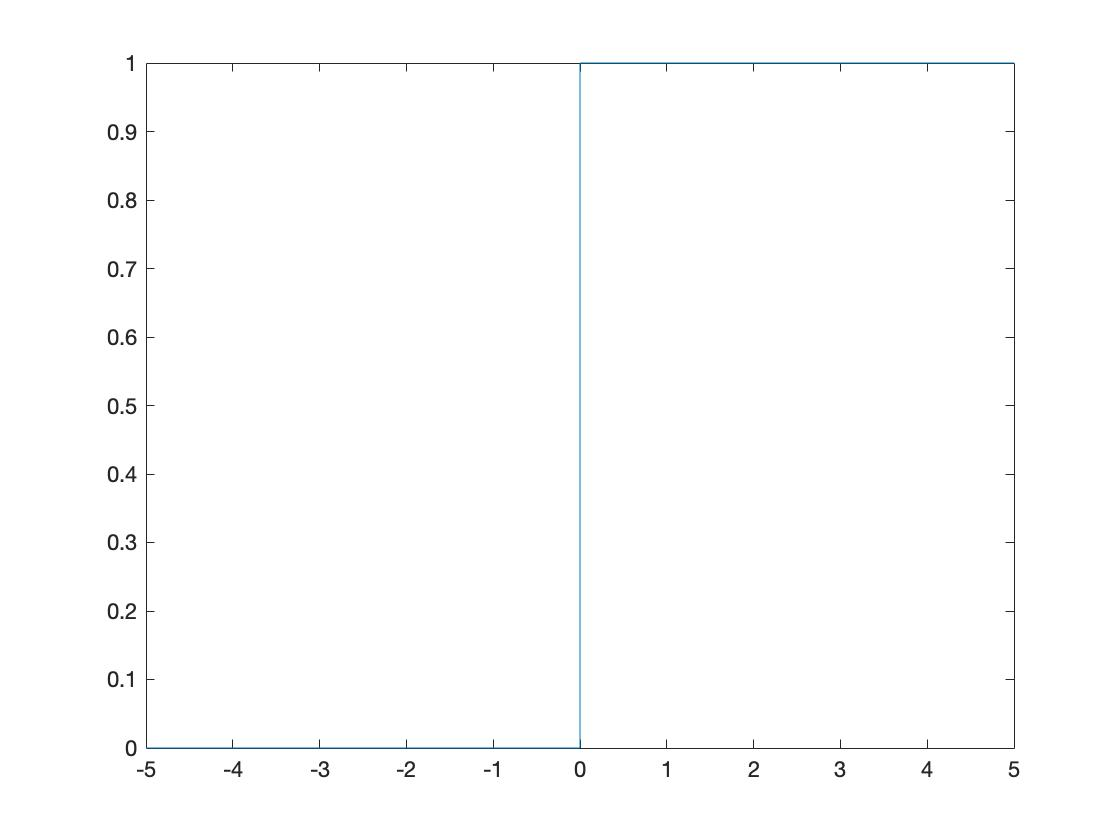
\includegraphics[width=14cm]{2.jpg}
    \caption{单位阶跃函数}
\end{figure}

(3)正弦信号
\begin{equation}
    y=\sin{t}
\end{equation}

\begin{lstlisting}
%% sinusoidal signal
t=-5:0.01:5;
y=sin(t);
plot(t,y);
ylim([-2 2]);
\end{lstlisting}
\begin{figure}[H]
    \centering
    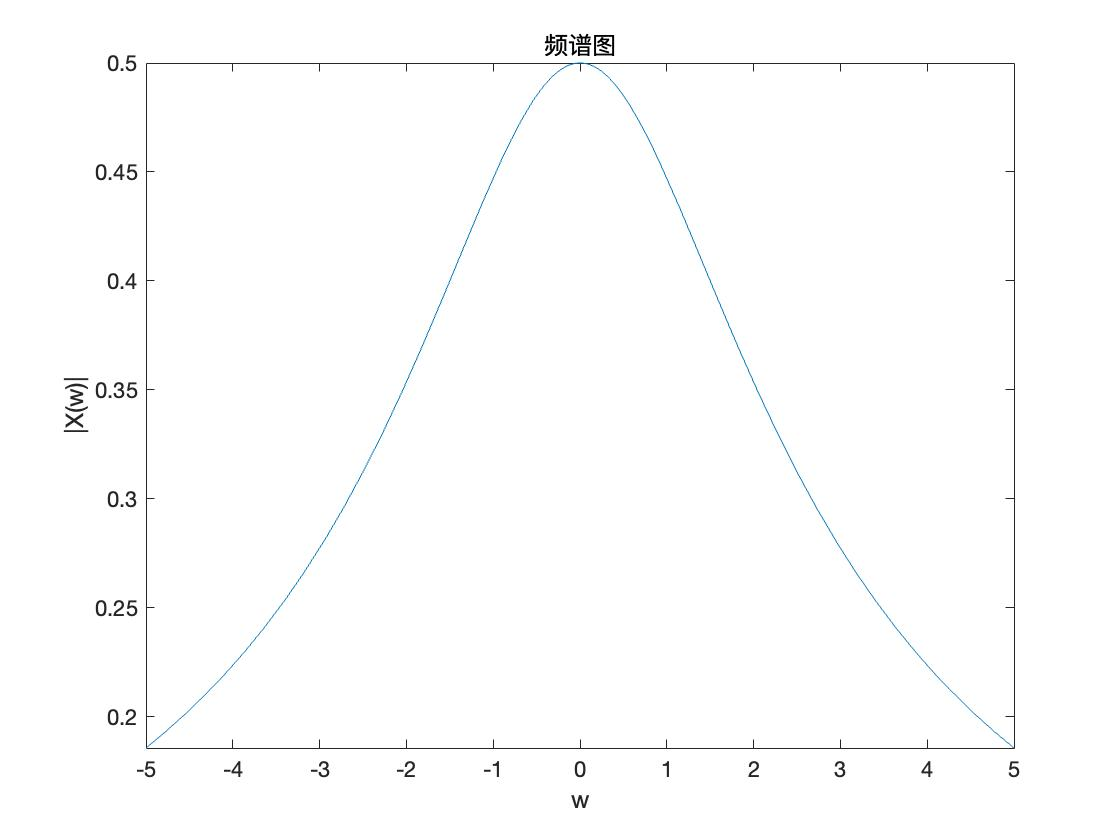
\includegraphics[width=14cm]{3.jpg}
    \caption{正弦信号}
\end{figure}

(4)$[-2,2]$区间内的指数信号$e^{-2t}$
\begin{equation}
    y=e^{-2t}
\end{equation}

\begin{lstlisting}
%% Exponential signal
t=-2:0.01:2;
y=exp(-2*t);
plot(t,y);
\end{lstlisting}
\begin{figure}[H]
    \centering
    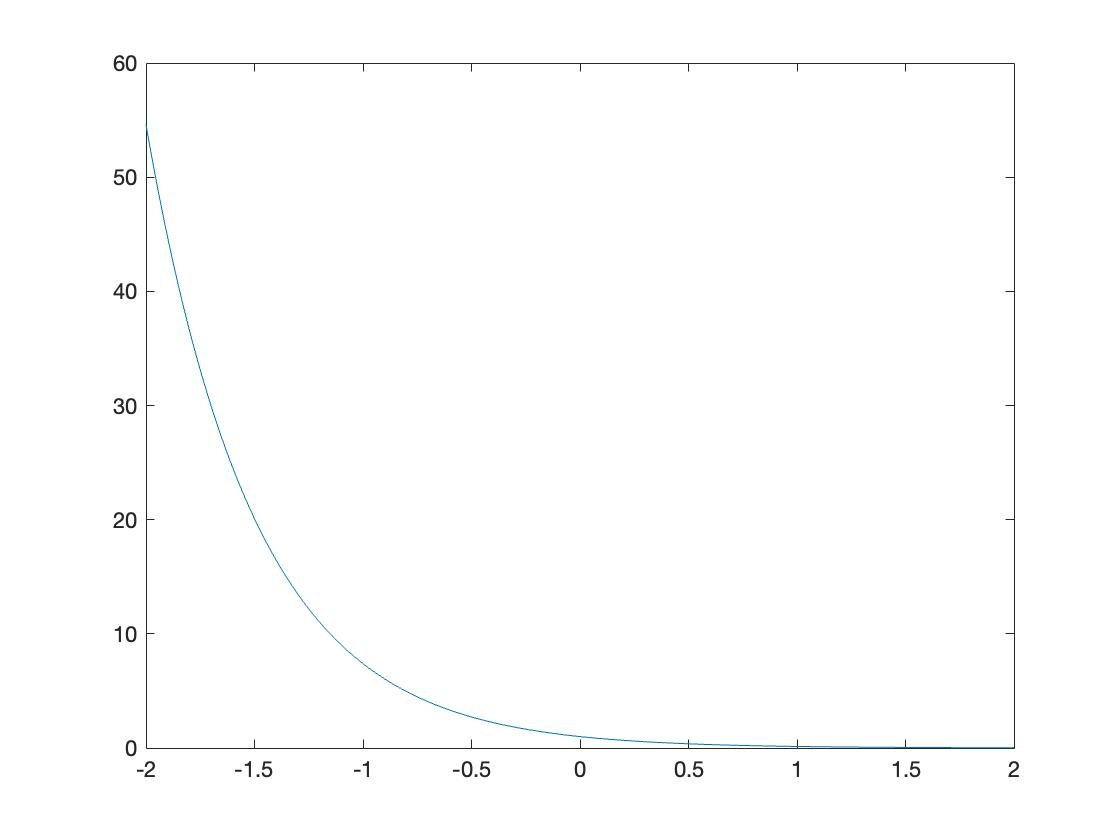
\includegraphics[width=14cm]{4.jpg}
    \caption{$[-2,2]$区间内的指数信号$e^{-2t}$}
\end{figure}

(5)周期三角波和锯齿波
\begin{lstlisting}
%% Periodic triangular wave
t=-5:0.01:5;
y=sawtooth(2*pi*t,0.5);
plot(t,y);
ylim([-2 2]);

%% Periodic sawtooth wave
t=-5:0.01:5;
y=sawtooth(2*pi*t,1);
plot(t,y);
ylim([-2 2]);
\end{lstlisting}
\begin{figure}[H]
    \centering
    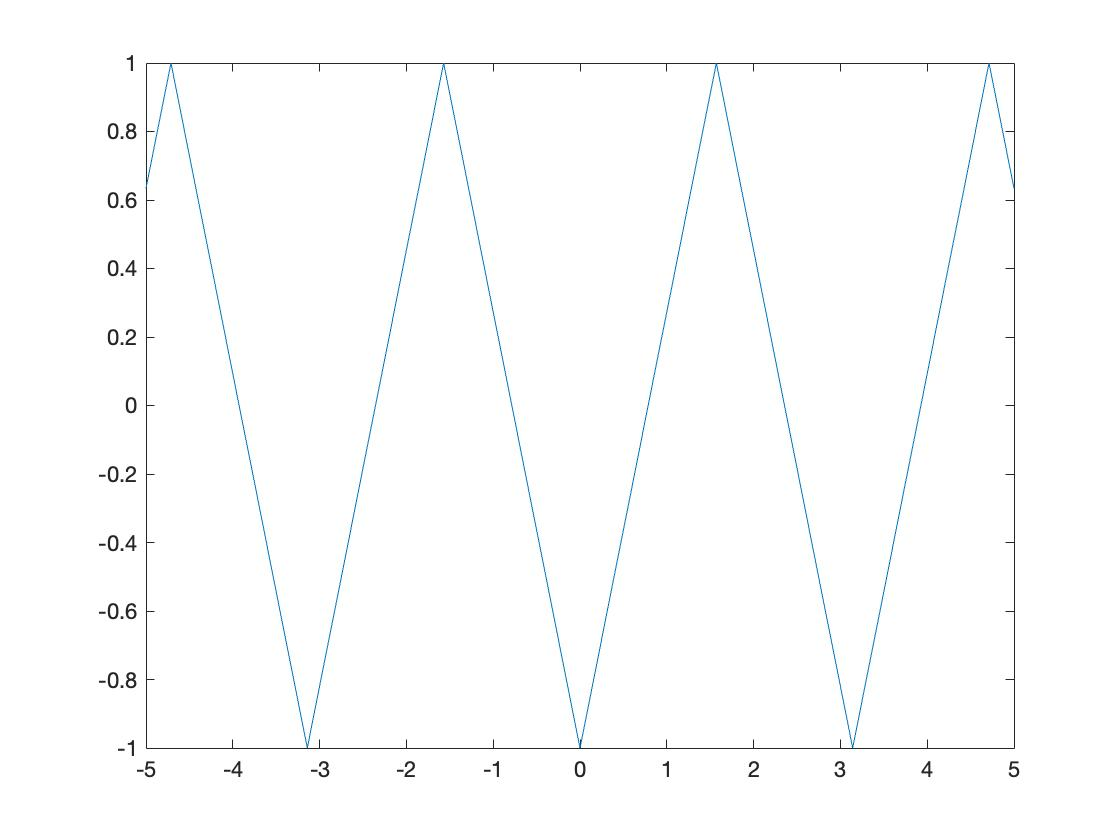
\includegraphics[width=14cm]{5.jpg}
    \caption{周期三角波}
\end{figure}
\begin{figure}[H]
    \centering
    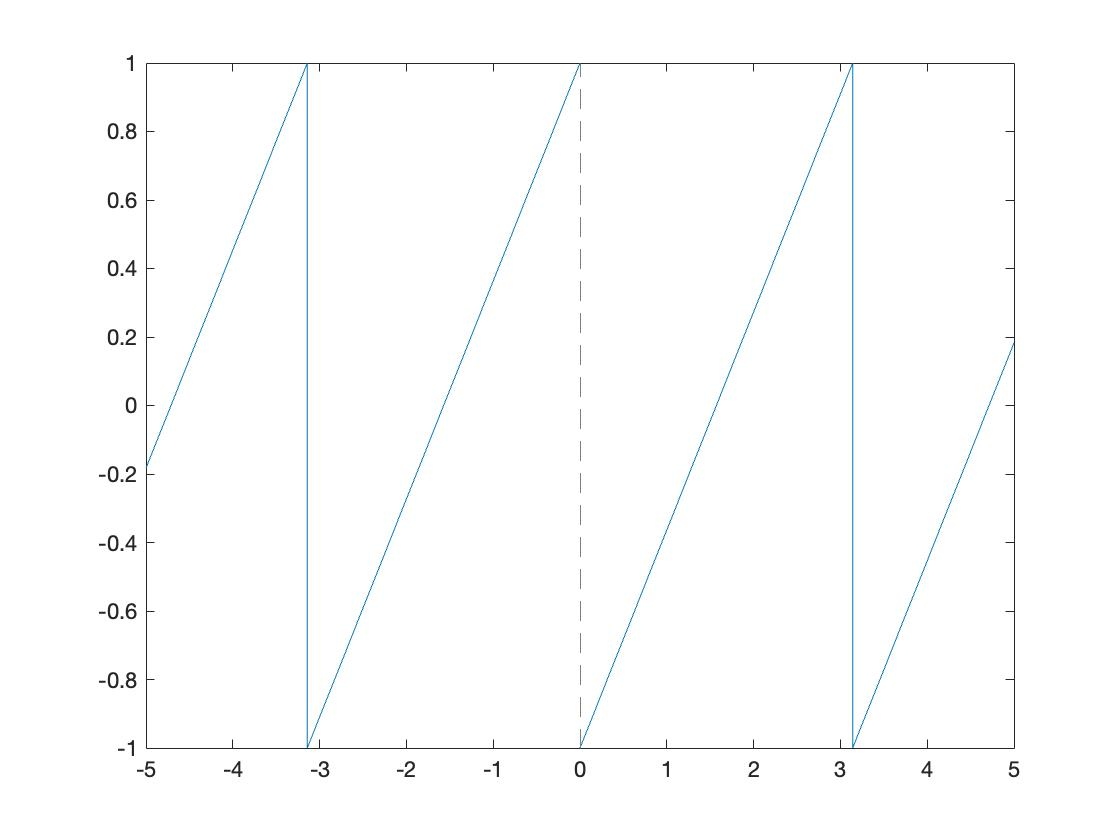
\includegraphics[width=14cm]{6.jpg}
    \caption{周期锯齿波}
\end{figure}

(6)周期方波
\begin{lstlisting}
%% Periodic square wave
t=-5:0.01:5;
y=square(2*pi*t);
plot(t,y);
ylim([-2 2]);
\end{lstlisting}
\begin{figure}[H]
    \centering
    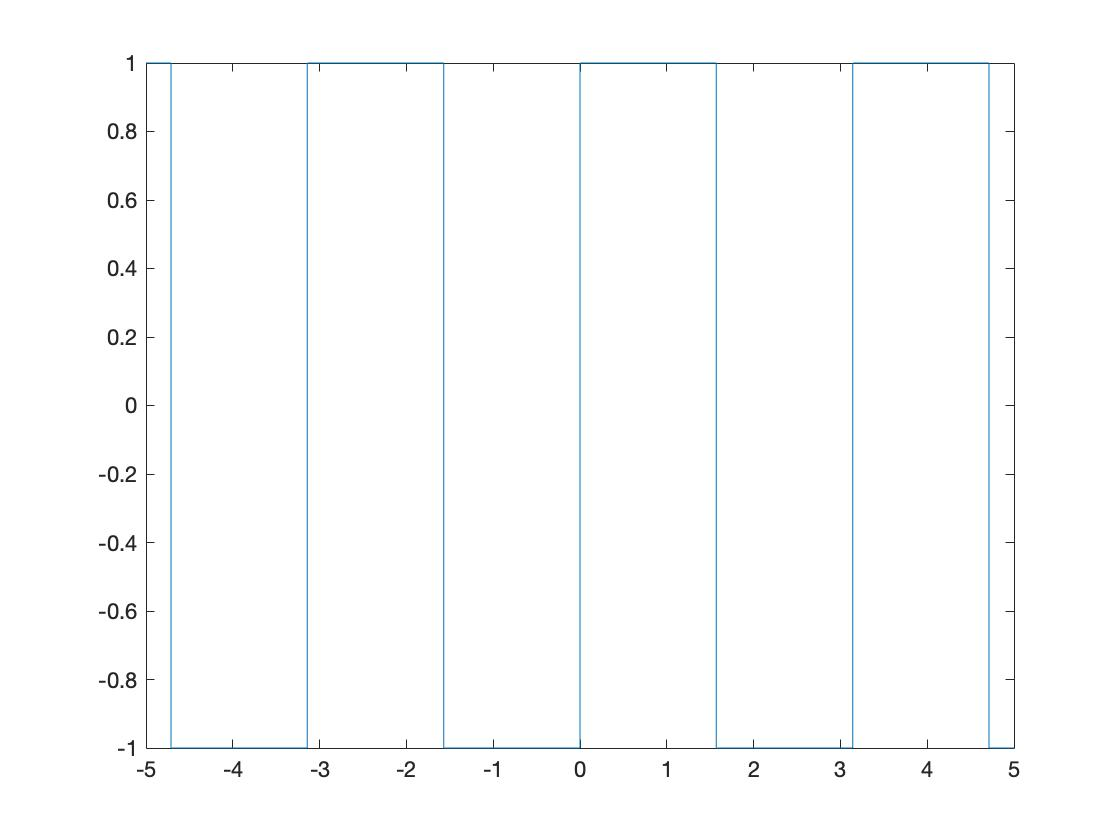
\includegraphics[width=14cm]{7.jpg}
    \caption{周期方波}
\end{figure}

(7)$[-4\pi,4\pi]$区间内的采样信号$Sa(t)$
\begin{lstlisting}
%% Sampling signal Sa(t)
t=-4*pi:0.01:4*pi;
y=sin(t)./t;
plot(t,y);
\end{lstlisting}
\begin{figure}[H]
    \centering
    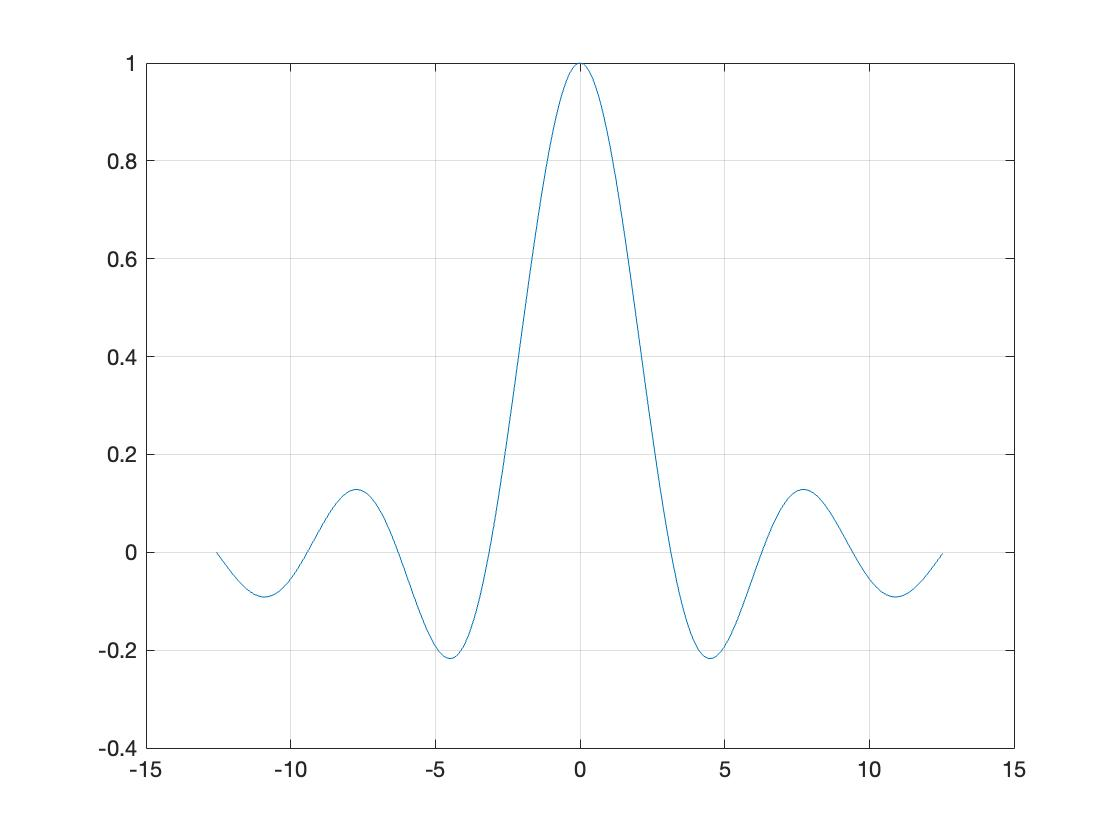
\includegraphics[width=14cm]{8.jpg}
    \caption{$[-4\pi,4\pi]$区间内的采样信号$Sa(t)$}
\end{figure}

\leftline{2. 已知信号}
\begin{equation}
    \left\{\begin{matrix}
        0.25(t+4) & -4<t<0 \\
        1         & 0<t<2  \\
        0         & others
    \end{matrix}\right.
\end{equation}
\par
用尺度变换法分步画出$x(-2t+4)$的波形图。

翻转+时间轴展缩平移+平移,运算过程如图所示,即:
\begin{equation}
    x(t)\rightarrow x(-2t)\rightarrow x[-2(t-2)]=x(-2t+4)
\end{equation}

\begin{figure}[H]
    \centering
    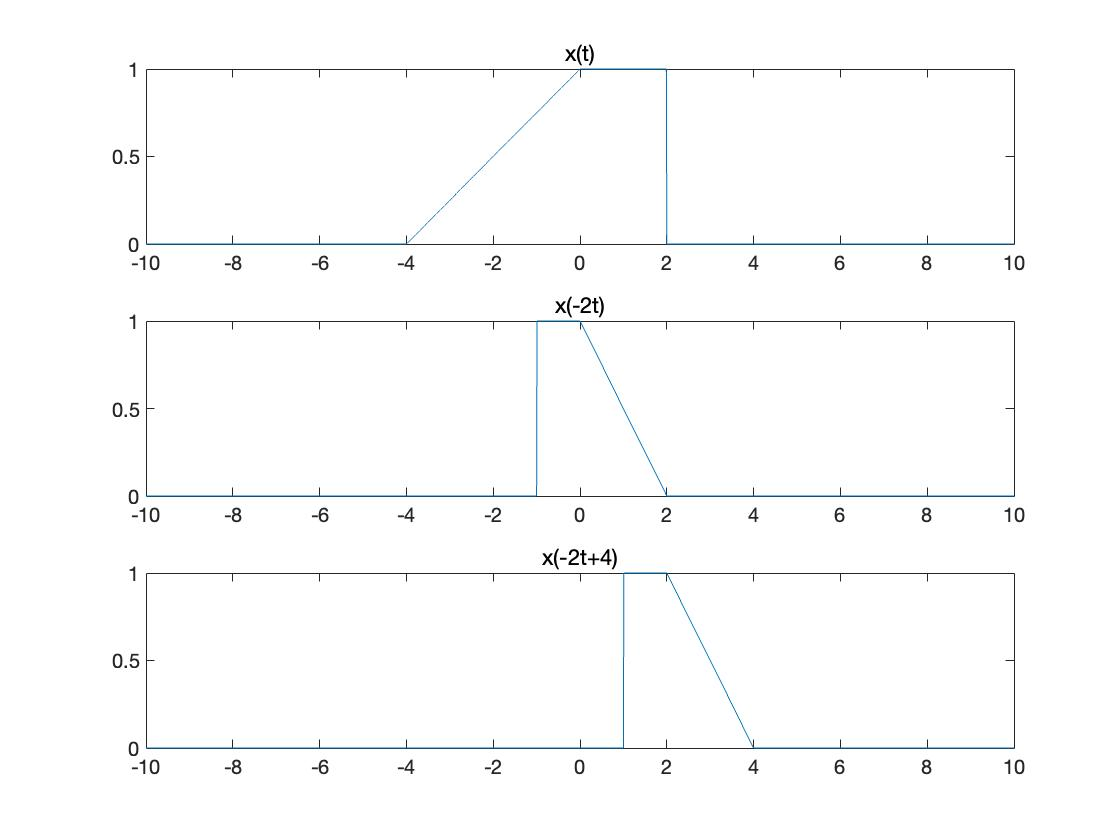
\includegraphics[width=14cm]{2_new.jpg}
    \caption{变换过程}
\end{figure}


\leftline{3. 求信号$x(t)=e^{-2t}$的傅立叶变换并画出频谱图。}
由于$x(t)$不满足狄利赫里条件,应乘上一个单位阶跃函数。
\begin{equation}
    x(t)=e^{-2t}u(t)
\end{equation}
\begin{lstlisting}
% problem 3
clc,clear
%% Fourier transform
syms t w;
X=fourier(exp(-2*t)*heaviside(t))
fplot(abs(X));
\end{lstlisting}
经过傅里叶变换得:
\begin{equation}
    X(\omega)=\frac{1}{2+\omega i}
\end{equation}
\begin{figure}[H]
    \centering
    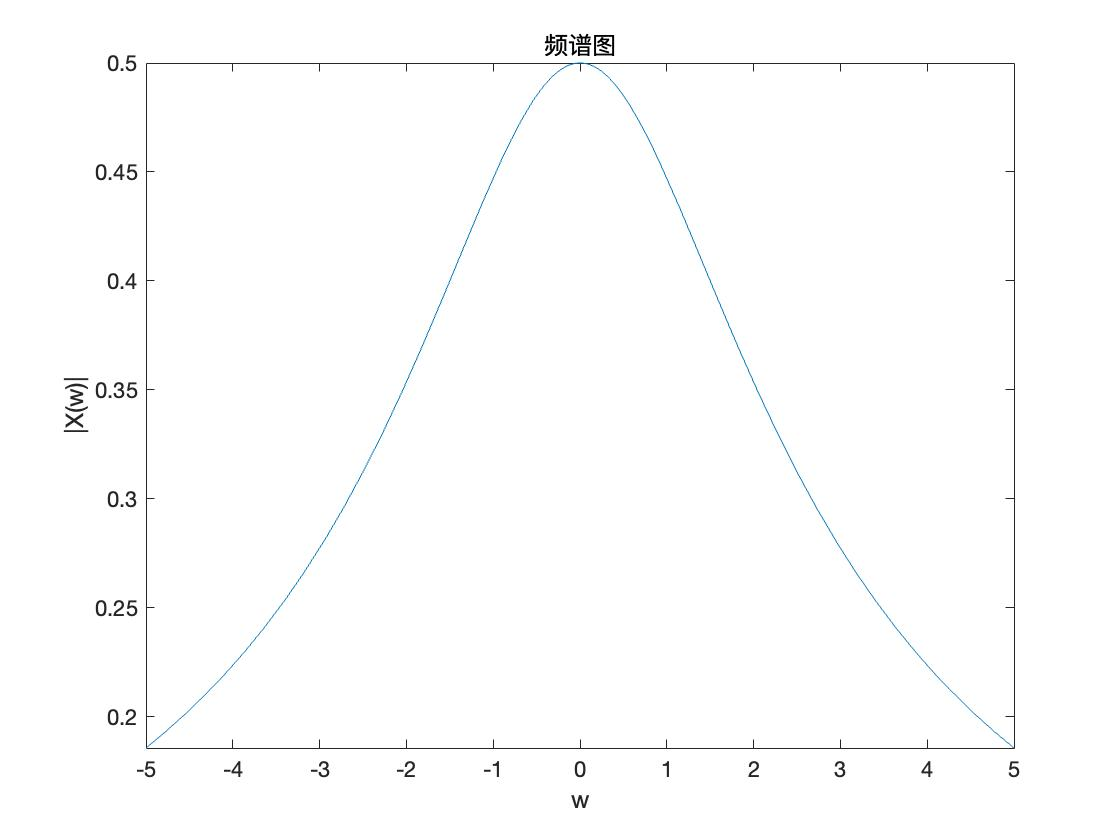
\includegraphics[width=14cm]{3.jpg}
    \caption{频谱图}
\end{figure}


\leftline{4. 求$X(\omega)=e^{-\frac{\omega ^2}{4}}$的傅立叶反变换$x(t)$并画出波形图。}
\begin{lstlisting}
% problem 4
syms w;
xt=ifourier(exp(-w^2/4))
fplot(xt);
\end{lstlisting}
经过傅里叶逆变换得:
\begin{equation}
    x(t)=\frac{e^{-x^2}}{\sqrt{\pi}}
\end{equation}
\begin{figure}[H]
    \centering
    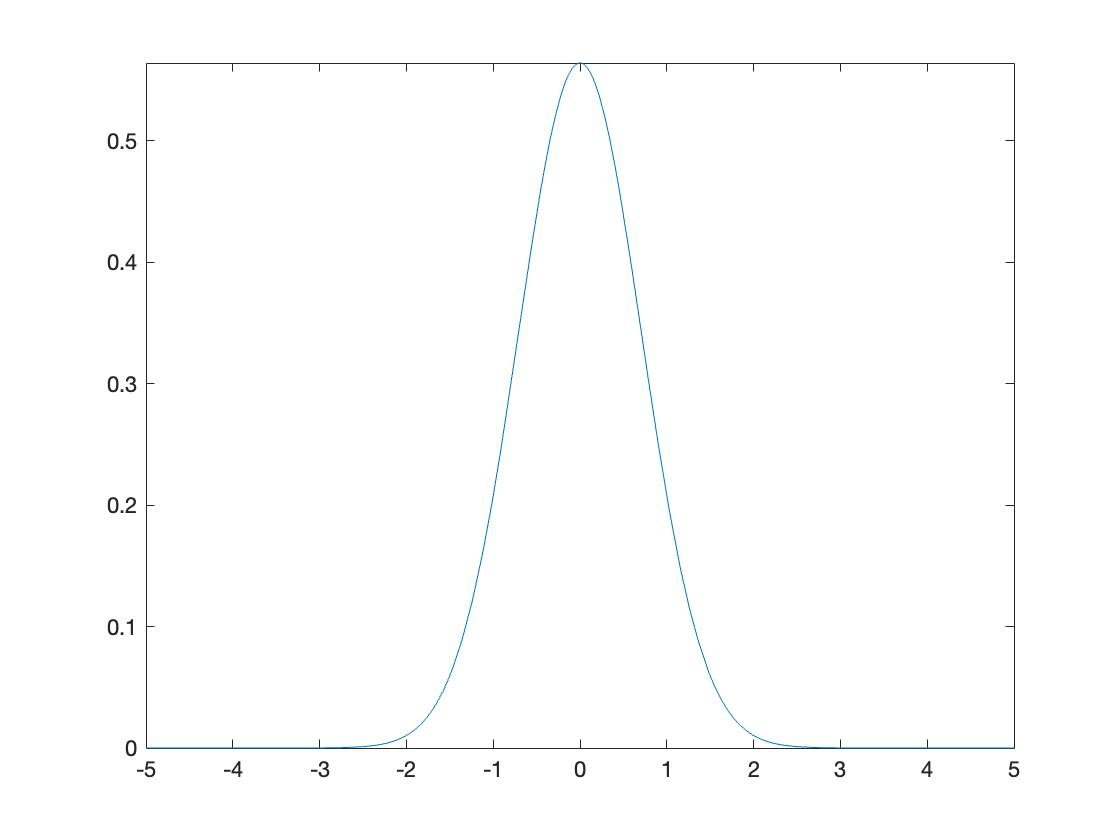
\includegraphics[width=14cm]{4_1.jpg}
    \caption{$x(t)$波形图}
\end{figure}

\leftline{5. 求信号$x(t)=e^{-3t}cos(t)u(t)$的拉普拉斯变换。}
\begin{lstlisting}
% problem 5
syms t;
L=laplace(exp(-3*t)*cos(t)*heaviside(t))
fplot(L);    
\end{lstlisting}
经过拉普拉斯变换得:
\begin{equation}
    F(s)=\frac{s+3}{(s+3)^2+1}
\end{equation}
\begin{figure}[H]
    \centering
    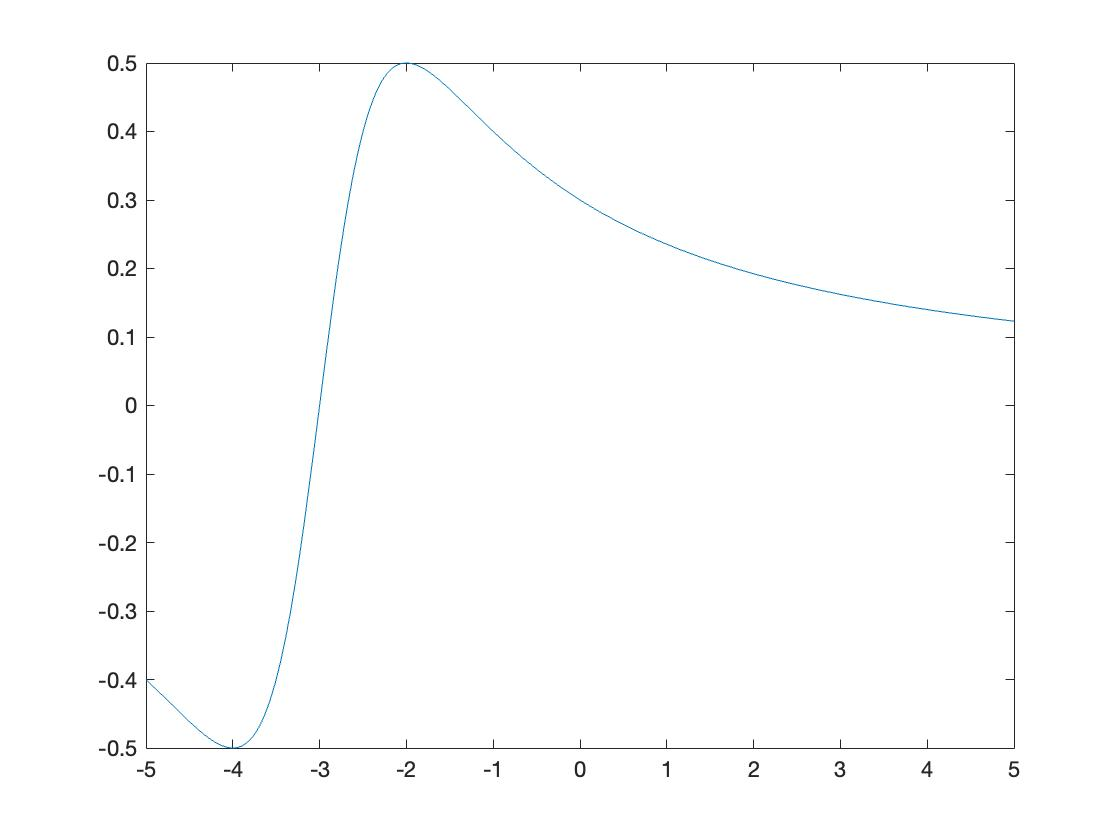
\includegraphics[width=14cm]{5_1.jpg}
    \caption{$F(s)$波形图}
\end{figure}

\leftline{6. 求$X(s)=\frac{s}{s^2+2s+1}$的拉普拉斯反变换。}
\begin{lstlisting}
% problem 6
syms s;
x=ilaplace(s/(s^2+2*s+1))
fplot(x);    
\end{lstlisting}
经过拉普拉斯反变换得:
\begin{equation}
    x(t)=e^{-t}-te^{-t}
\end{equation}
\begin{figure}[H]
    \centering
    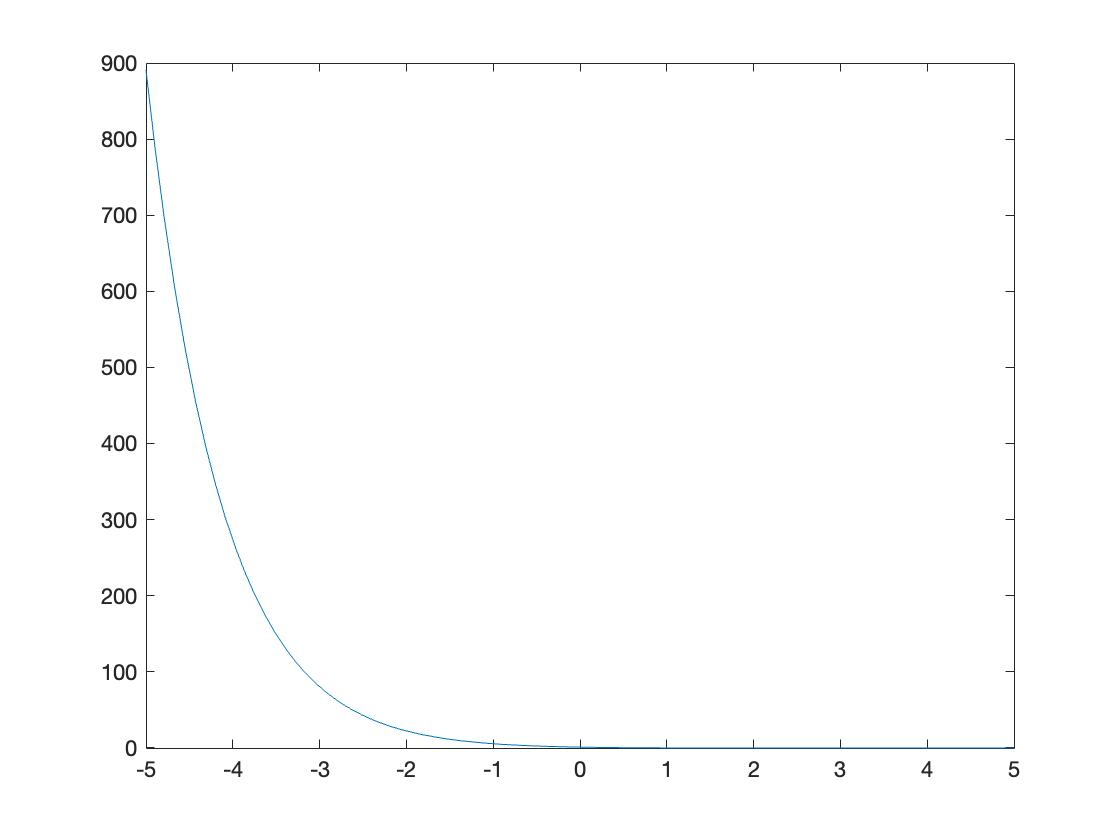
\includegraphics[width=14cm]{6_1.jpg}
    \caption{$x(t)$波形图}
\end{figure}

\leftline{7. 求任意三角波的微分和积分运算并画出波形图。}
\begin{lstlisting}
% problem 7
clc,clear
%% Primitive function
step=0.001;
t=-10:step:10;
x=@(t)(sawtooth(t,0.5));
x_i=zeros(size(t));
subplot(3,1,1);
plot(t,x(t));

%% Integral operation
for i=1:size(t,2)
    x_i(i)=integral(x,-10,t(i));
end
subplot(3,1,2);
plot(t,x_i)

%% Differential operation
x_dt=diff(x(t))./step;
subplot(3,1,3);
plot(t(2:end),x_dt)
\end{lstlisting}

\begin{figure}[H]
    \centering
    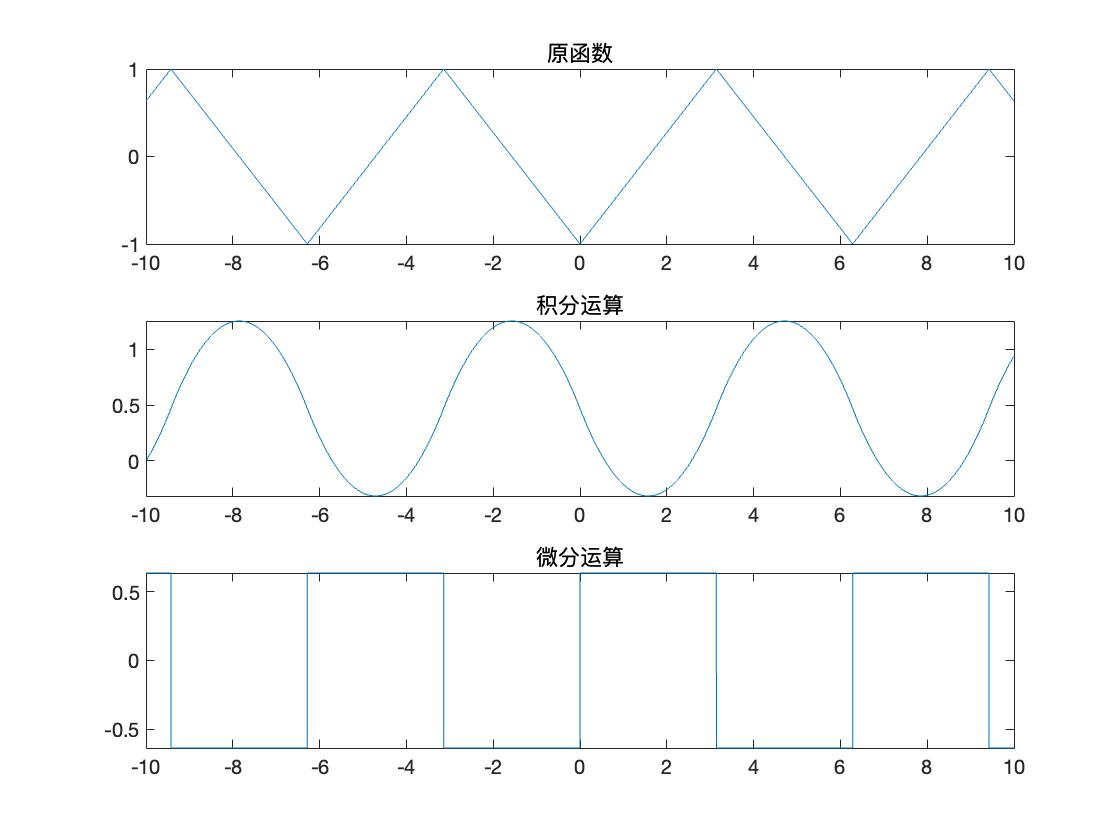
\includegraphics[width=14cm]{7_new.jpg}
    \caption{运行结果}
\end{figure}

\leftline{\textbf{小结:}}
\par
通过本次实验,我了解了连续时间信号的基本概念及其运算实现,
熟悉了Matlab编程特点,建立了对连续时间信号及其频谱的直观认识。
在本次实验中,我一开始只会用向量形式离散地表示一个函数,后来
听了老师的直播后发现可以用$fplot()$和$ezplot()$函数自动地
绘制出函数曲线。同时,在第二问用尺度变换法求波形图时,我学会了
分段函数的一种新的表示方法,即用逻辑值与该段函数值相乘再求和。
同时,我学会了用$subplot()$函数将多个图像显示在一张图中,
大大提升了清晰度,简化了表达。
\par
在最后一问求任意三角波的微分和积分运算并画出波形图中,我发现
$sawtooth()$函数无法将syms类型连续变量当做自变量,后来我使用
离散向量形式,成功画出了积分和微分运算图。
\par
总得来说,经过了本次实验,我对上课所学知识有了更深层次的理解,
初步学会了Matlab的基本操作,为日后学习打下了坚实的基础。
\end{document}